\documentclass[10pt,twocolumn,a4paper]{article}

\usepackage[margin=1.4cm]{geometry}
\usepackage{graphicx}
\usepackage{amsmath,amssymb}
\usepackage{booktabs}
\usepackage{caption}
\usepackage{subcaption}
\usepackage{hyperref}

% Tighter section spacing
\usepackage{titlesec}
\titlespacing*{\section}{0pt}{0.8em}{0.3em}
\titlespacing*{\subsection}{0pt}{0.5em}{0.2em}
\titleformat{\section}{\normalsize\bfseries}{\thesection}{0.5em}{}
\titleformat{\subsection}{\small\bfseries\itshape}{\thesubsection}{0.5em}{}

% Tighter captions
\captionsetup{font=small, skip=3pt}

\begin{document}

\begin{center}
{\Large\bfseries Intro to ML --- Milestone 2 Report}\\[0.6em]
{\footnotesize
\begin{tabular}{c c c}
Darius Giannoli & Stella Arsie & Ludovica Marcon \\
(380759) & (398286) & (390805)
\end{tabular}}
\end{center}

\section{Introduction}

Milestone~2 (MS2) returns to the Gaming and Mental Health dataset
($2000$ synthetic samples, $13$ behavioural features) introduced in
Milestone~1 (MS1) and reopens the same two questions: predict the
continuous addiction score (regression) and the 3-class addiction level
\{Low, Medium, High\} (classification). MS1 used linear regression, linear
classification and $k$-Nearest-Neighbours and concluded that the signal
was near-linear in the $13$ z-scored features. MS2 puts that conclusion
under stress by adding a non-linear parametric model --- a
Multi-Layer Perceptron (MLP) trained from scratch with
back-propagation --- and a fundamentally different family ---
K-Means used as a voting classifier. Class imbalance (Low~$68.9\%$,
Medium~$27.9\%$, High~$3.2\%$) keeps macro-F1 as the primary
classification metric; mean squared error (MSE) is the regression
metric. Hyperparameters are selected by 5-fold cross-validation (CV).

\section{Methodology}
\subsection{Data \& Preprocessing}
We z-score normalize the $13$ features using \emph{training-set}
statistics only. Crucially, we shuffle the training data with a fixed
random seed \emph{before} taking an $80/20$ train/validation split,
removing the leakage risk that an ordered split would otherwise
introduce (an issue we did not handle in MS1). The validation split is
used for hyperparameter selection only; the final test set
($N{=}400$) is held out until the very last evaluation.

\subsection{Validation protocol}
For classification we use stratified 5-fold CV --- the High class has
only $n{\approx}41$ training samples, so non-stratified folds risk
empty validation slices. We report mean and standard deviation across
the five folds. Hyperparameters are selected by the highest CV
macro-F1 (and not by classification error rate); for K-Means we also
report the within-cluster sum of squares (inertia) to compare init
strategies on their native objective.

\section{Methods \& Results}

\subsection{Multi-Layer Perceptron}
\label{sec:mlp}
We implement a fully-connected MLP with arbitrary depth, ReLU or
sigmoid activations, and an output layer chosen by task: Softmax with
Cross-Entropy (CE) loss for classification, Identity with MSE for
regression. Forward and backward passes are coded by hand; the
optimiser is mini-batch Stochastic Gradient Descent (SGD) with optional
heavy-ball momentum ($\beta$). Weights are initialised with the
Glorot/Xavier scheme ($\sigma{=}\sqrt{2/(\text{fan-in}{+}\text{fan-out})}$)
to avoid the gradient-vanishing collapse reported in the lecture
slides.

\emph{Hyperparameter sweeps.} We swept the learning rate $\eta$ on a
log grid from $10^{-4}$ to $10^{-1}$ (Fig.~\ref{fig:mlp}a) and the
hidden architecture across six choices ranging from a single hidden
layer with $32$ units to a $3$-layer pyramid of $(128,\,64,\,32)$
units (Fig.~\ref{fig:mlp}b). The lr curve is sharply peaked: F1
collapses for $\eta\!\lesssim\!10^{-3}$ (too few effective steps in
40~epochs) and degrades mildly for $\eta\!\geq\!10^{-2}$
(noisier updates), with the best CV F1 at $\eta{=}3{\cdot}10^{-3}$.
The architecture sweep is essentially flat
(all six configurations within $0.03$~F1 of one another and
within fold standard deviation), which mirrors the MS1 finding that
the regression signal is near-linear: adding width or depth does not
unlock any usable non-linearity. We therefore select the smallest
network --- one hidden layer with $32$ ReLU units --- as the simpler
solution.

\emph{Selected configuration.} One hidden layer of $32$ ReLU units,
$\eta{=}3{\cdot}10^{-3}$, momentum $\beta{=}0.9$, batch size $32$,
$40$ epochs. The training curve (Fig.~\ref{fig:mlp}c) converges
smoothly to a final-epoch validation CE of $0.33$.

\begin{figure}[t!]
    \centering
    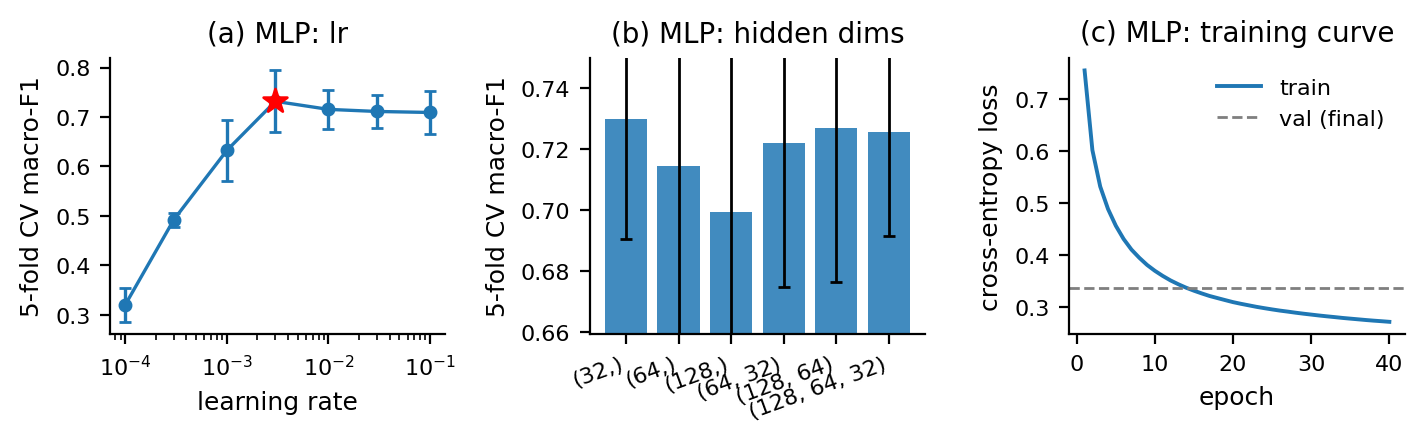
\includegraphics[width=\columnwidth]{figures/mlp_summary.png}
    \vspace{-0.3cm}
    \caption{MLP sweeps (5-fold stratified CV macro-F1, error bars are
    fold std). \textbf{(a)} Learning rate $\eta$ (log-$x$); red star =
    selected value. \textbf{(b)} Hidden-layer architecture; flat curve
    within fold noise. \textbf{(c)} Training cross-entropy of the
    selected model vs the final-epoch validation value (grey dashed).}
    \label{fig:mlp}
\end{figure}

\subsection{K-Means voting classifier}
\label{sec:kmeans}
K-Means partitions the training set into $K$ clusters by iteratively
assigning points to their nearest centre (Euclidean distance) and
re-computing centres as cluster means. To use it as a classifier we
attach a label to each cluster by majority vote over its training
points, then classify a new point as the label of its nearest cluster.
We implement two creativity extensions: K-Means++ seeding (each new
centre sampled with probability proportional to its squared distance to
the nearest existing centre) and best-of-$N$ restarts (run the
algorithm $N$ times, keep the lowest-inertia solution).

\emph{Choosing $K$.} The number of clusters $K$ controls a strong
tension on this dataset (Fig.~\ref{fig:km}a). Inertia decreases
monotonically with $K$ (no clear elbow), but \emph{F1} keeps rising
up to $K{=}30$ then degrades at $K{=}50$. The reason is class
imbalance: with $K{=}3$ a majority vote inside each cluster collapses
to the global majority (Low), giving accuracy~${\approx}70\%$ but
macro-F1~$0.27$. Increasing $K$ creates smaller, locally purer
clusters where Medium and High samples can dominate, lifting
minority-class recall. We select $K{=}30$.

\emph{Initialisation does not matter for F1.}
Fig.~\ref{fig:km}b sweeps four init strategies at the selected $K$,
$20$ random seeds each: K-Means++ and best-of-$10$ restarts both
reduce the inertia variance ($\sigma{\approx}17$ for
\textit{km++}{$\times$}$10$ vs $\sigma{\approx}46$ for plain random),
confirming they do find geometrically better optima. But all four
strategies land within $0.03$~F1 of one another, all within their own
seed-to-seed std ($\sim\!0.07$). The K-Means objective (inertia) and
the downstream classifier objective (macro-F1) are simply not aligned
once cluster labels are decided by voting on imbalanced classes.

\begin{figure}[t!]
    \centering
    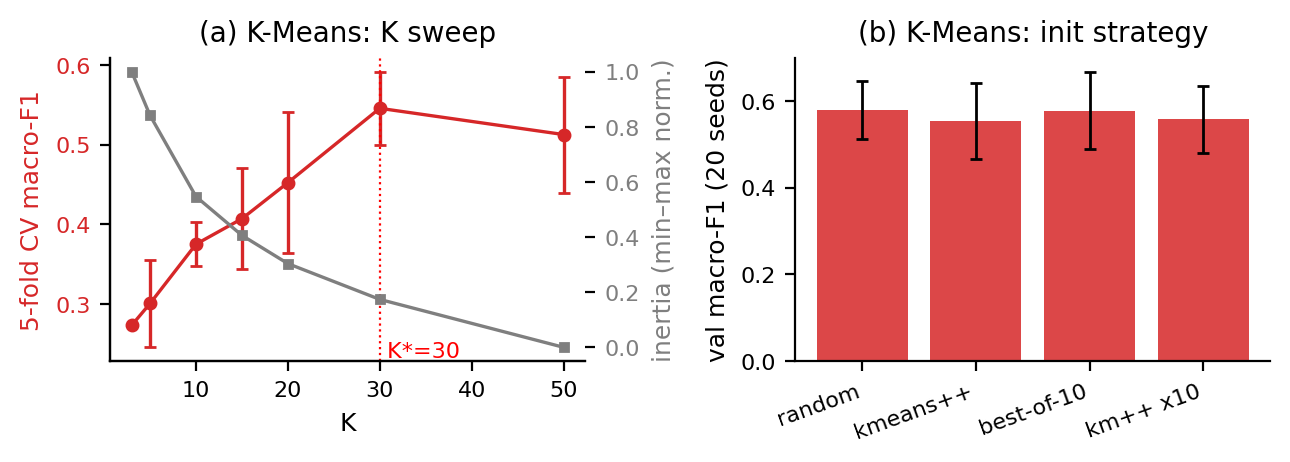
\includegraphics[width=\columnwidth]{figures/kmeans_summary.png}
    \vspace{-0.3cm}
    \caption{K-Means sweeps. \textbf{(a)} $K$ sweep: 5-fold CV
    macro-F1 (red) versus normalised inertia (grey). The inertia
    elbow ($K{\approx}15$) disagrees with the F1 peak ($K{=}30$),
    reflecting the imbalanced-vote effect discussed in
    §\ref{sec:kmeans}. \textbf{(b)} Init strategy at $K{=}30$,
    $20$ random seeds: better inertia does not translate to better F1.}
    \label{fig:km}
\end{figure}

\section{Discussion \& Conclusion}

\subsection{MS2 vs MS1: which family wins?}
\label{sec:vs}
Fig.~\ref{fig:cmp} and Table~\ref{tab:final} consolidate every
selected MS1 and MS2 model on the same held-out test set. Three
take-aways stand out.

\emph{MLP beats every MS1 classifier.} On classification, the small
MLP reaches test macro-F1 $\mathbf{0.798}$, a clear $+0.07$ over MS1's
best (Linear SVM at $0.733$). This contradicts the surface reading of
the MS1 conclusion that the signal is near-linear. The two
observations reconcile if one looks at \emph{where} the gain comes
from: MS1 already noted that minority-class recall was the bottleneck.
The MLP's Softmax+CE combination, trained with class-aware
back-propagation, fits a smoother probability surface in the High
neighbourhood than the hinge-loss SVM. The architecture sweep
(Fig.~\ref{fig:mlp}b) shows the MLP does \emph{not} use width or depth
for new non-linear features --- those plateau within fold noise ---
so the residual signal it picks up is loss-driven, not
representation-driven.

\emph{MLP regression matches ridge within noise.} For regression,
the MLP gives test MSE $1.101$ vs MS1's closed-form ridge ($0.993$);
the gap is within the fold-to-fold variation observed during CV.
Without a structural non-linearity to exploit, the more flexible model
carries no advantage over a $14$-parameter ridge that was already
optimal on this data.

\emph{K-Means is comparable to $k$-NN but well below parametric
methods.} The voting classifier achieves test F1 $0.603$, within
$0.02$ of MS1's $k$-NN ($0.623$) --- which is the same order of
magnitude as the $\sim\!0.08$ seed-to-seed std we observed in
Fig.~\ref{fig:km}b --- but $0.19$ below the MLP. Both K-Means and
$k$-NN partition feature space by geometric proximity rather than by
class boundaries, so neither matches the parametric supervised models
on this imbalanced task.

\begin{figure}[t!]
    \centering
    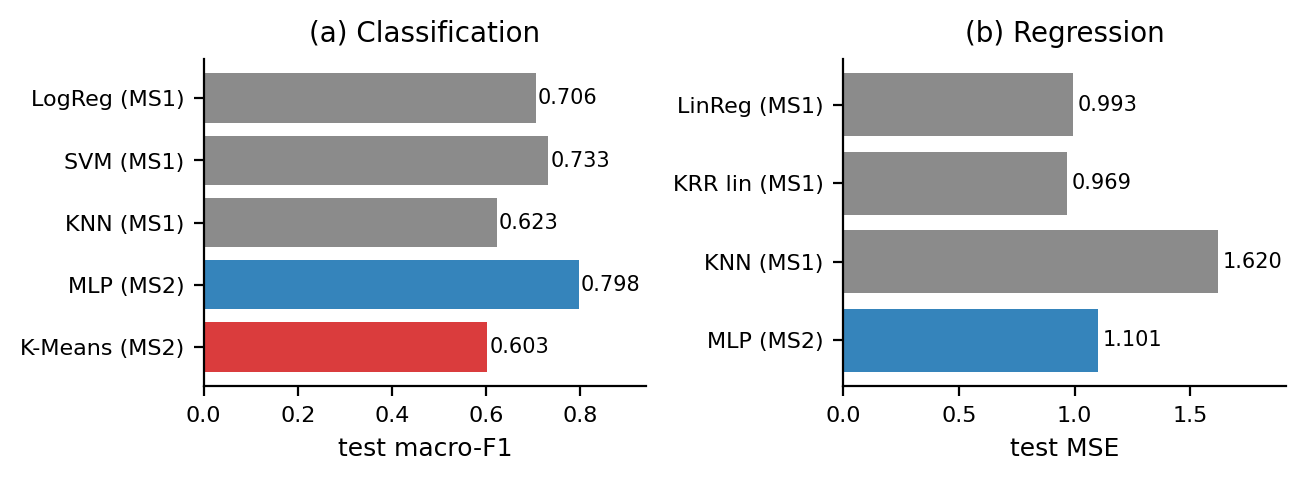
\includegraphics[width=\columnwidth]{figures/comparison.png}
    \vspace{-0.3cm}
    \caption{Final test-set comparison (gray = MS1 models, blue = MS2
    MLP, red = MS2 K-Means). \textbf{(a)} macro-F1 (higher = better).
    \textbf{(b)} MSE (lower = better).}
    \label{fig:cmp}
\end{figure}

\subsection{Conclusion}
\label{sec:conclusion}
A from-scratch MLP with a small hidden layer of $32$ ReLU units and
heavy-ball momentum gives the best classifier we have produced across
both milestones (test F1 $\mathbf{0.798}$); the gain over MS1's SVM
comes from a smoother loss surface around the minority class, not
from any new representational capacity. On regression the MLP merely
matches MS1's ridge solution within fold noise, consistent with the
near-linear signal in the $13$ z-scored features. K-Means used as a
voting classifier is competitive with $k$-NN but trails every
parametric supervised model; we also observe that choosing $K$
matters far more than how clusters are initialised --- a
counter-intuitive finding that we trace to the misalignment between
the K-Means inertia objective and the imbalanced voting objective.

\begin{table}[h]
\centering
\caption{Selected configurations and test-set performance across the
two milestones. Reg: MSE (lower = better); Clf: accuracy /
macro-F1 (higher = better). Best of each task in bold.}
\label{tab:final}
\resizebox{\columnwidth}{!}{%
\begin{tabular}{llll}
\toprule
\textbf{Method} & \textbf{Task} & \textbf{Config} & \textbf{Test} \\
\midrule
\textbf{LinReg (MS1)} & reg & CF ridge $\lambda{=}10$        & MSE $\mathbf{0.993}$ \\
KRR (MS1)      & reg & linear kernel, $\lambda{=}1$         & MSE $0.969$ \\
KNN (MS1)      & reg & $k{=}17$, cosine, weighted           & MSE $1.62$  \\
MLP (MS2)      & reg & $(32)$, $\eta{=}3{\cdot}10^{-3}$, $\beta{=}0.9$ & MSE $1.101$ \\
\midrule
LogReg (MS1)   & clf & balanced wts, $\eta{=}0.3$, $\beta{=}0.9$ & $80.4\%$ / F1 $0.706$ \\
SVM (MS1)      & clf & $\lambda{=}10^{-2}$, batch $32$         & $82.3\%$ / F1 $0.733$ \\
KNN (MS1)      & clf & $k{=}17$, cosine, weighted              & $80.1\%$ / F1 $0.623$ \\
\textbf{MLP (MS2)} & clf & $(32)$ ReLU, Softmax+CE, $\beta{=}0.9$ & $86.3\%$ / F1 $\mathbf{0.798}$ \\
K-Means (MS2)  & clf & $K{=}30$, km++${\times}10$              & $72.8\%$ / F1 $0.603$ \\
\bottomrule
\end{tabular}}
\end{table}

\end{document}